\chapter{Rezultati}
\section{Delitev podatkov}
Za končno raziskavo smo imeli na voljo 7368 primerov stanj iz podatkovne zbirke EEG Motor Movement/Imagery Dataset. Primere stanj smo skrčili na enakomerno razporeditev, z 2456 primeri vsakega stanja. Sami smo posneli neka minut posnetkov, 186 primerov stanj od tega 62 primerov vsakega stanja. Za učenje nevronskih mrež smo uporabljali množice za učenje z 75\% podatkov in množice za testiranje z 25\% podatkov.



\section{Rezultati na MMID}
\subsection{Classification learner}
Z uporabo aplikacije clasifiacation learner smo testirali več načinov klasifikacije. Dosegli so naslednje natančnosti:
\begin{table}[h]
\centering
\begin{tabular}{|c|c|}
\hline
Metoda klasifikacije & natančnost \\
\hline
odločitvena drevo & 40\% \\
\hline
k-NN & 41\% \\
\hline
logistična regresija & 49\% \\
\hline
SVM & 45\% \\
\hline
nevronska mreža & 51\% \\
\hline
\end{tabular}
\caption{Natančnosti klasifikacij}
\end{table}

\begin{figure}[h!]
\begin{center}
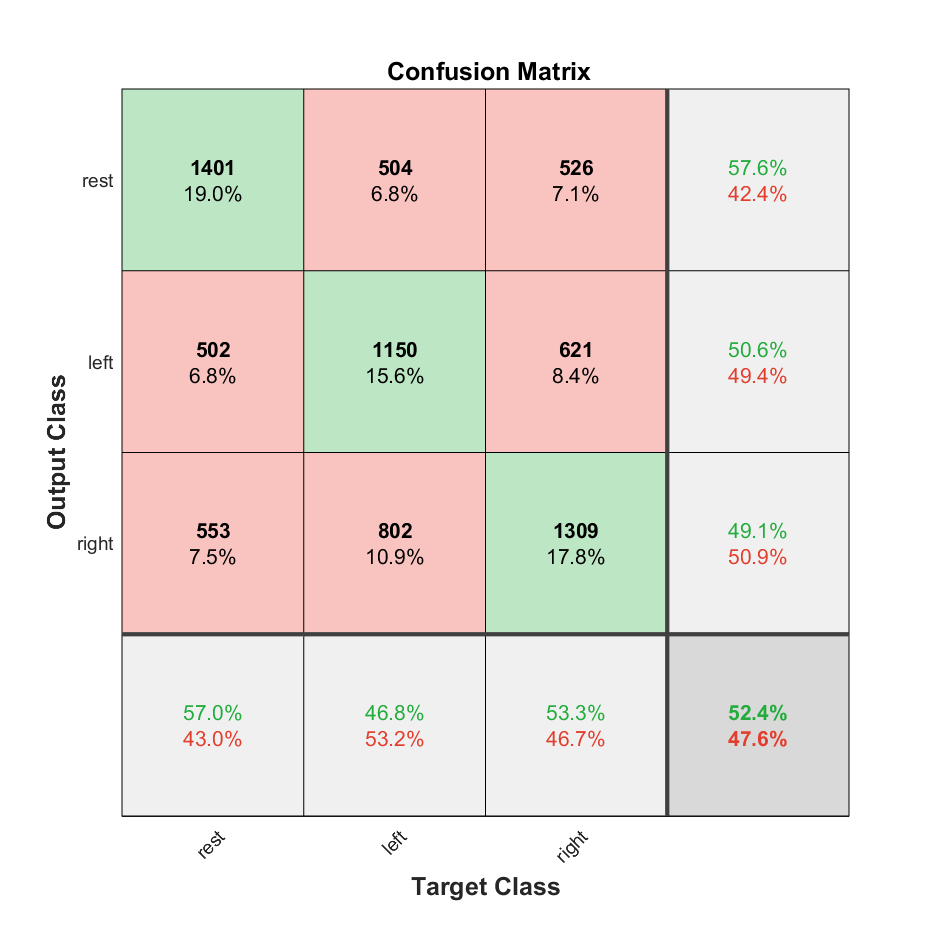
\includegraphics[width=0.5\linewidth]{slike/Confusion_13-20Hz_0s-4s.png}
\end{center}
\caption{Matrika zmede nevronske mreže.}
\end{figure}



\section{Rezultati na lastnih podatkih}
S svojimi podatki smo dodatno naučili nevronsko mrežo. Ker se naprave na katerih so podatki snemani razlikujejo je natančnost klasifikacije padla na 42\%
\begin{figure}[h!]
\begin{center}
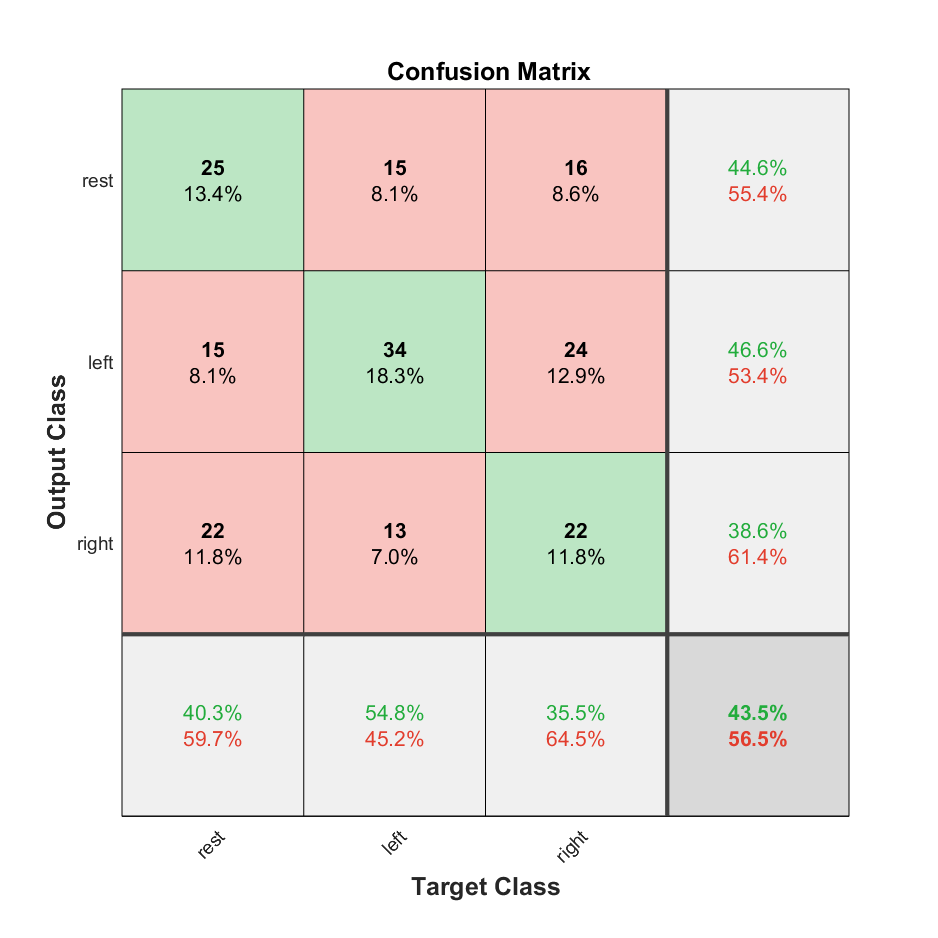
\includegraphics[width=0.5\linewidth]{slike/Confusion_13-20Hz_0s-4s_retrained.png}
\end{center}
\caption{Natančnost klasifikacije na lastnih podatkih.}
\end{figure}
\section{Preizkus v realnem času}

\section{Primerjava funkcij}
Da bi preverili ali filtra vrneta enake rezultate z našimi metodami, smo uporabili povezljivostno metodo CPCC na območju beta in naučili nevronski mreži na podatkih filtriranih z funkcijo eeglaba in filtrom ki smo ga uporabili za implementacijo v realnem času. Obe nevronski nevronski mreži sta imeli 54\% natančnost.
\begin{figure}[h!]
\begin{center}
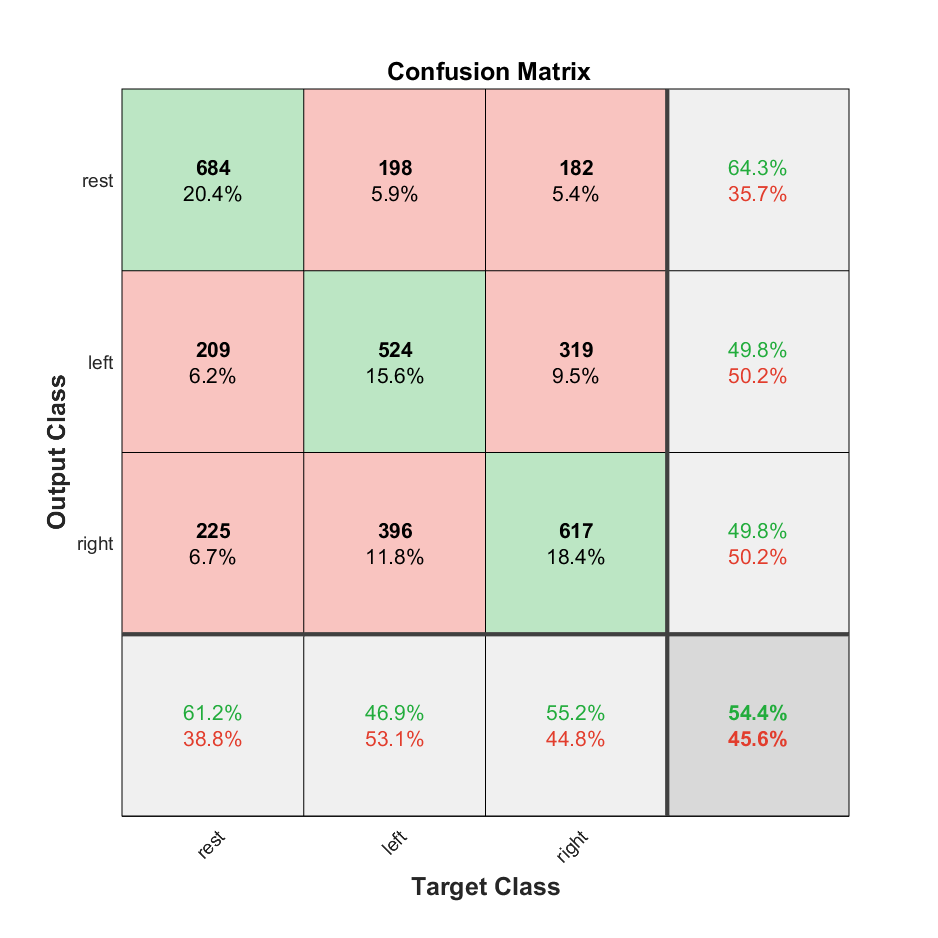
\includegraphics[width=0.5\linewidth]{slike/Confusion_eeglab.png}
\end{center}
\caption{EEGLAB filtriranje.}
\end{figure}

\begin{figure}[h!]
\begin{center}
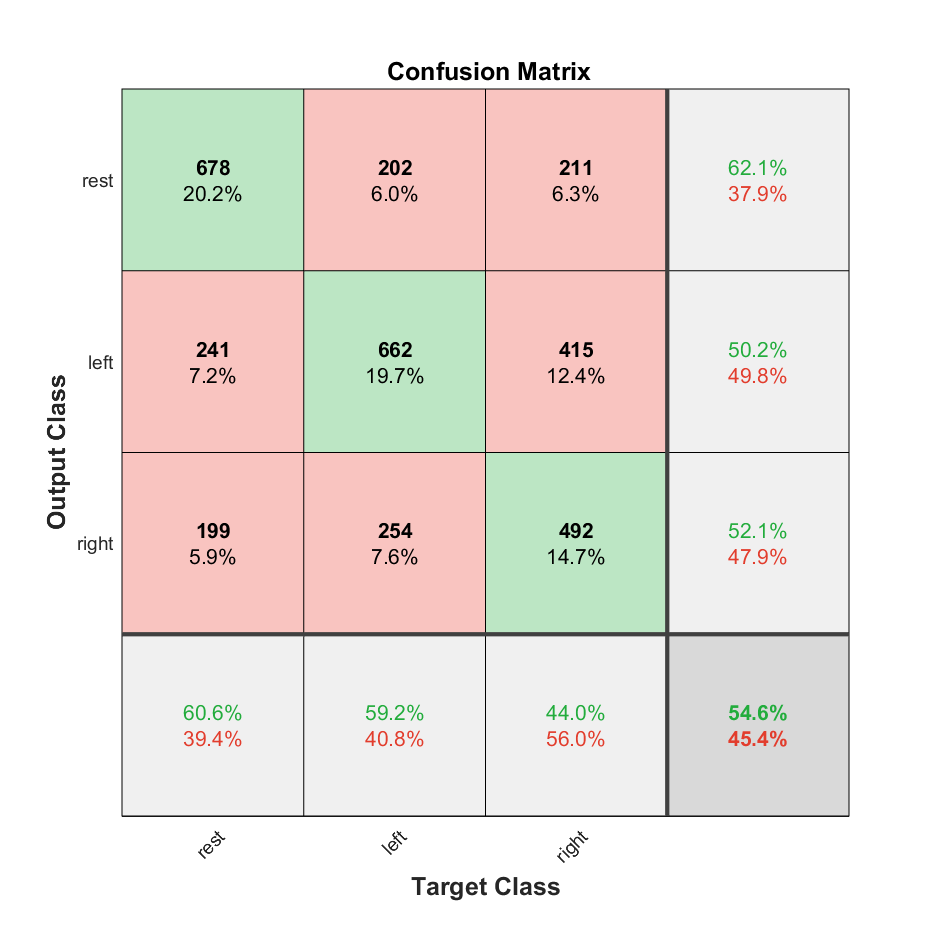
\includegraphics[width=0.5\linewidth]{slike/Confusion_my.png}
\end{center}
\caption{Filtriranje v realnem času.}
\end{figure}


